\documentclass[11pt]{article}
\usepackage{graphicx}
\usepackage[margin=0.75in]{geometry}

\graphicspath{ {image/} }

\title{Report}
\author{
  Chang, Zheng\\
  \texttt{changzheng1993}
  \and
  Escobar, Giancarlo\\
  \texttt{giancarloescobar}
  \and
  Pimentel, Noel\\
  \texttt{noelpimentel}
  \and
  Yousuf, Imran\\
  \texttt{imranyousuf}
}

\bibliographystyle{siam}

\begin{document}
\maketitle

\abstract{The functional architecture of the object vision pathway in the human 
brain was 
investigated using fMRI imaging to measure patterns of response in ventral 
temporal cortex while subjects viewed categories of objects in Haxby et al. 
[Science 293 (2001) 2425] \cite {haxby2001vt}. Haxby argued that 
category related responses in the 
VT lobe during visual object identification were overlapping and distributed in 
topography. At the time of Hanson et al. [Elsevier 23 (2004) 156] \cite 
{hanson2004combinatorial} there were prevailing views that objects codes were 
focal and localized to specific areas like the fusiform and the parahippocampal 
gyri.  Hanson et al. revisited the Haxby data and provided a crucial test of 
the former hypothesis using a neural network classifier.  The method of Hanson 
et al. detected more general topographic representations and illustrated that 
substantially the same VT lobe voxels contribute to classification of all 
object categories
}

\section{Introduction}

\setlength{\parskip}{10pt}

Models for the functional architecture of the ventral temporal cortex fall into 
three categories. One model proposes that VT contains a limited number of areas 
that are specialized for representing specific categories of stimuli. A second 
model proposes that different areas in VT are specialized for different types 
of perceptual processes. The third model proposes that the representations of 
faces and different categories of objects are widely distributed and 
overlapping.  According to the latter model, VT has a topographically organized 
representation of attributes of form that underlie face and object recognition 
meaning that the representation of a face or object is illustrated by a unique 
pattern of response across a wide expanse of cortex in which primary and 
secondary regions (i.e. large- and small-amplitude responses) hold information 
about face and object appearance.

Haxby et al. tested this model by investigating the patterns of response evoked 
in the ventral temporal cortex by faces and multiple categories of objects 
(face, house, cat, bottle, scissors, shoe, chair, scrambled image) in a series 
of runs on six subjects. Patterns of response were defined as those voxels with 
response that differed significantly by category and will be referred to as POR 
for future purposes. The data \cite{haxby2001vor} were analyzed to determine 
whether the stimulus category that a subject was viewing could be identified on 
examining the similarity between the POR evoked by each category on even and 
odd runs. Within-category correlations and between-category correlations were 
compared to determine whether a POR to one category, such as chairs, could be 
distinguished from the pattern of response to a different category, such as 
shoes, with and without the exclusion of maximally responsive voxels. For the 
inclusion of maximally responsive voxels, The POR in object-selective ventral 
temporal cortex correctly identified the category being viewed in 96 percent of 
pairwise comparisons. Identification accuracy for faces, houses, and scrambled 
pictures was at 100 percent and identification accuracy for the small man-made 
objects (bottles, scissors, shoes, and chairs) was significantly better than 
chance for each category. For the exclusion of maximally responsive voxels, for 
example, within the cortex that responded maximally to houses, the POR 
correctly identified the category being viewed with 93 percent accuracy, 94 
percent for small man made objects, and 83 percent for faces.  These results 
demonstrate that POR in VT carries information about the type of object being 
viewed, even in cortex that responds maximally to other categories.

The work by Hanson et al. established Haxby et al. results while further 
extending the original analysis.  Hanson et al. neural network classifier 
detected more general topographic representations and achieves an 83 percent 
correct generalization performance on patterns of voxel response in 
out-of-sample tests.  Using voxel-wise analysis Hanson et al. showed that the 
same VT lobe voxels contribute to the classification of all object categories, 
suggesting that the code is combinatorial as Haxby et al. suggested. Our own 
analysis will adhere to the methods of Haxby et al. and Hanson et al. with the 
plan of reproducing the Haxby similarity method (comparisons between 
within-category correlation and between-category correlation) and reproducing 
and improving upon the POR classification rate with a neural network and 
homogenous methods. We will make the these studies reproducible in the sense 
that code used to obtain said results will be easily understandable and 
readable by others; any graph, statistics, etc. from these studies can be 
easily simplified and reproduced with the aid of well documented executable and 
readable code.

\section{Data}

The data consists of 64 slices  64 X 40 BOLD collected from a GE 3T (repetition 
time = 2500 ms, forty 3.5-mm-thick sagittal images, field view of = 24 cm, echo 
time = 30 ms, flip angle = 90 percent). Patterns of neural response were 
measured with functional magnetic resonance imaging (fMRI) in six subjects 
while they viewed pictures of faces, cats, five categories of manmade objects. 
Twelve time series were obtained for each subject. Each time series began and 
ended with 12-s rests and contained eight stimulus blocks of 24-s duration, one 
for each category, separated by 12-s interval of rest. Stimuli were presented 
for 500 ms with an inter stimulus interval of 1500 ms. Repetitions of 
meaningful stimuli were pictures of the same face or object photographed from 
different angles; stimuli for each meaningful category were four images each of 
12 different exemplars. The data shape for any particular run is (40, 64, 64, 
121) that can be read as 64 slices 64 X 40 BOLD for 121 contiguous slices in 
time (i.e. 121 volumes of time).

\section{Preprocessing}

\subsection{Masking}

Since our fMRI data is represented as a 4D block of data, we are interested in 
working on the voxel time-series in the brain. It is then necessary to apply a 
mask on the 4D brain images to subset the voxels in the brain that we will be 
analyzing.

\subsection{Smoothing}

fMRI data has a low signal-to-noise ratio. Any reduction of random noise in the 
image will imporve the ability to detect true activation.  For this reason, 
smooth has become a commonly used pre-processing step in the analysis of fMRI 
data. Smoothing the data will improve our signal to noise ratio by applying a 
small blurring kernel across the image.

\section{Methods}

\subsection{Linear Model}
Ideally we want to detect any signal in relation to a task i.e. we want to 
determine which voxels contain high activation based on BOLD response to 
stimulus, (e.g. house, face, cat, shoe, house, scrambled, chair, bottle). We 
may detect signal by subtracting task from rest or by calculating a correlation 
between the task-on / task-off vector and the voxel time course. However, by 
using a Generalized Linear Model to fit our fMRI time series data, we will able 
to calculate a unique weight for each voxel that represents the different level 
of activation across all the voxels that we can use to distinguish BOLD 
response per stimulus.  We will regress the BOLD time series across all voxels 
against the timing and duration of each stimuli (8 predictors) The GLM for our 
fMRI data is:

y? =X?? +??

Y is our BOLD signal, X the design matrix with our predictors, B the that 
describe the relationship between the predictors and response, and E the 
unexplained noise in the BOLD data.

\subsection{Design}
Before we performed a regression analysis, we masked the data in order to 
distinguish the voxels that are in the brains versus the voxels that are 
outside the brain. Before applying a mask on subject001 run001 (fig X), we took 
the mean volume (over time) (3D brain image) and plotted a histogram of the 
mean volume values. (Fig x). By selecting the correct threshold, we will be 
able identify the voxels inside the brain, a 3D brain mask. We first selected a 
threshold of 1100. We then carelessly looped through each subject and run and 
applied the same threshold of 1100 only to conclude that threshold will differ 
between subjects and their runs (Figs X-Z: histogram showing different 
thresholds are needed). 

		Figs X-Z (hist) and brain images using the same threshold

To effectively solve this problem, we used FUNCTION that provides an algorithm 
that computes a unique threshold, therefore a unique mask, for each subject and 
run. This method was more efficient and accurate as we showed that the voxels 
within the brain slightly vary  across subjects and their runs. Here are the 
resulting brain images (fig a-c), same as (fig x-z), but with a unique mask for 
each run. We can clearly see the algorithm has  more accurately selected the 
voxels in the brain. Now that we?ve removed on average 700,000 voxels per run, 
we can now perfomm a regression analysis on the subset of voxels that are in 
the brain.    
          
\subsection{Hemodynamic Response}

Our design matrix consists of 8 predictors, representing the ideal time series 
that represent what we think the response should look like to each of the eight 
stimulus.. Ideally we want to know the activation at the neuronal level but 
this is beyond the capability of fMRI, for we don’t know when that signal 
is occurring other than the time intervals in which the subject is shown the 
stimuli. To account for this we have to convolve with the hemodynamic response 
function. Hemodynamic response (HDR) allows the rapid delivery of blood to 
active neuronal tissues. If a subject is shown a photo of a cat the brain will 
presumably receive a rapid delivery of blood to activate the neuronal tissues 
for identifying/processing cat. The probability density function of the gamma 
distribution
	
	         Gamma(r, lambda)

can model this situation and provide us with a continuous function that is 
close to the hemodynamic response we observe for a single brief event in the 
brain.

		Image of onsets blocks
		Image of onsets blocks with HDR

By using HDR to create the convolved regressors, we bridged through neural 
response and BOLD. These predictors will now closely simulate the onsets and 
allow our model to more accurately capture the changes in the BOLD activation 
associated with the presentation of stimulus to the subject.

This results to the following design matrix (X):

     Design Matrix with color bar  *describecolor bar*
     black=small value in regressor
     white = shows when the regressor is at the its largets value
     grey = intermediate values

Using the design matrix, we used least squares to estimate the B (beta coeff) by:

     Equation for solving for Betas under matrices

Thus, B hat will serve as the unique weights for each voxel. The beta 
coefficient gives us the amplitudes of the 8.

The B hat represents the parameter weight, or how much each regression factor 
contributes to the overall data. The B hat has the shape of (91,109, 91,8). 
Each slice across the fourth dimension yields a unique set of beta coefficients 
corresponding to that particular slice (i.e. stimuli). Additionally, slicing 
through the third dimension reveals the amplitude over the voxels through a 
transverse cut of the brain. The central slice can bee seen in Figure X for the 
first run for subject one.
For example, the following activation maps (Figures X,Y,Z) represent the beta 
coefficients (i.e the amplitude of each voxel) produced by the viewing of the 
object house, face, and scissors..

      Figure X = plt.imshow(betas vols[:,:,45,:])


Looking at the brain activation maps above, we can clearly see motion of the 
head in the scanner. 

\subsection{PCA}
Principal component analysis (PCA) is a standard tool in modern data analysis 
because it is a simple, non-parametric method for extracting relevant 
information about abstract and rather large data sets, such as fMRI.  Most 
import is that PCA is a significant tool for deriving a low-dimensional set of 
features from a large set of variables and can be used as a dimension reduction 
technique for regression on our design matrix. The linear and quadratic drift 
terms are able to model gradual drifts across the time-series but there are 
other patterns of noise, like brain anatomy, in our data that are undetectable 
by these methods. With PCA we can capture more of this noise and then remove 
these principle components by regression. The principle components are a 
sequence of projections, mutually uncorrelated and ordered in variance. In the 
our case the component vectors are the time-courses which provide a sequence of 
best linear approximations to our fMRI data.  Figure X illustrates the mutually 
uncorrelated projections ordered by variance.

	Figure X.

Many of the  components appear to explain much of the variance but we decided 
to examine the only first 10 as a rule of thumb.

	Figures 1-10 of projections

The first plot is the clearest and most obvious to contain brain anatomy rather 
than activation, for you can see the surrounding skull structure and the 
lateral ventricle. The other images were not so clear and for that we had to 
err on the side of caution. Plot 7 and 8 were on of the few images that 
displayed some sign of structure in the bottom right corner and top left 
corner, respectively.

\subsection{T-Map}
After getting the betas hat for each run from subject 001, we applied t statistics to look for the regions of the brain that reacts positively to the one category and negatively to the other category. First, we get the differences between two categories for each run and then reshape it from three dimension to one dimensions and concatenate the twelve runs. Therefore, we have runs by voxel matrix, which is two dimension.  Finally, we applied t-statistics to each voxel, and reshape the output back to three dimension. This process is called T-map.  Hence, the T-map can help us to investigate the regions of the brain that reacts positively to the one category and negatively to the other category. We also write a function for T-map, so it is very fast to get t-map for  each subject.


\subsection{House vs Face}

\begin{housevsface}
  \centering
    \reflectbox{%
      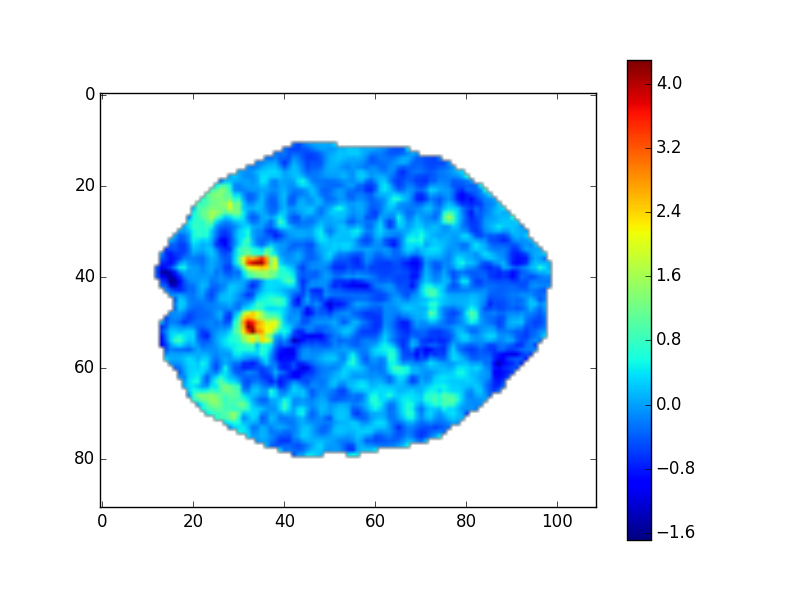
\includegraphics[width=0.9\textwidth]{2_PPA}}
    \caption{..................... Figure1: House vs Face}
           
           
First, I investigate the house and face.
According to the Figure, it is not hard to see that there are two red dots in the image. The two region  seem to react strongly to structure but not facial recognition. On the other hand, the  Therefore, I make a hypothesis: the two regions react strongly to structure. In order to test the hypothesis, we have to compare the house regressor and every other category regressor at the same scale. 
\end{housevsface}


\subsection{House vs Everything}

\begin{housevsface}
  \centering
    \reflectbox{%
      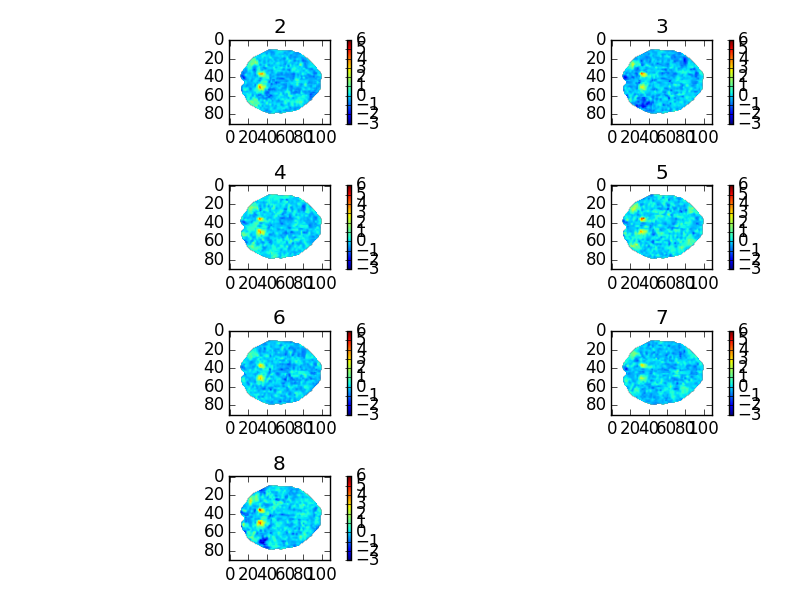
\includegraphics[width=1\textwidth]{house_everything}}
    \caption{Figure2: House vs Everything}
           
           
According to the graph, the hypothesis should be accepted because all of images have two red dot at the same spot. Therefore, the all graph has same type of structure. This shows that the two regions respond to much more house than other visual stimuli. According to the article “The Parahippocampal Place Area: Recognition, Navigation, or Encoding?”, it states that “The parahippocampal place area (PPA) has been demonstrated to respond more strongly in fMRI to scenes depicting places than to other kinds of visual stimuli.’ Based on this sentence, this is what we exactly found, and apparently the two regions are called parahippocampal place area (PPA). In conclusion, the PPA highly correlates to the structure such as house.
\end{housevsface}


\subsection{CAT1 and CAT2}

\begin{housevsface}
  \centering
    \reflectbox{%
      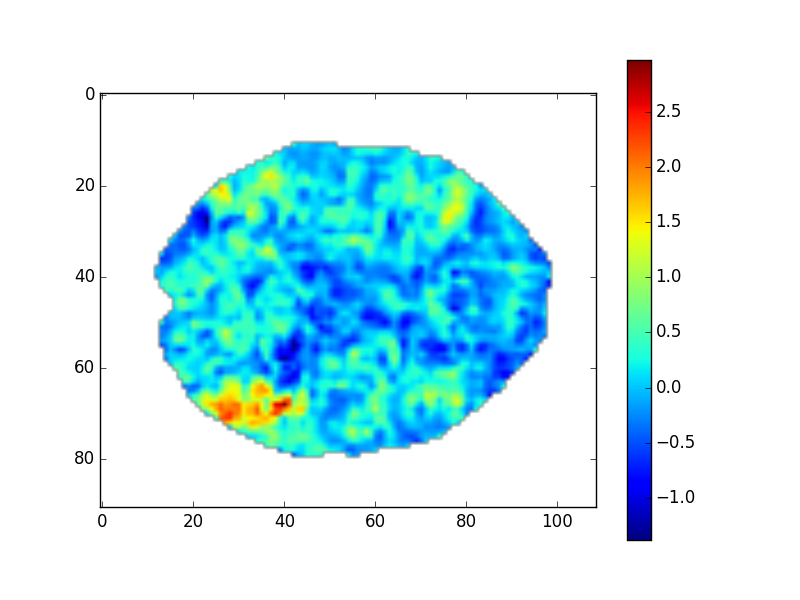
\includegraphics[width=0.7\textwidth]{2_CAT}}
    \caption{Figure3: CAT 1}
  \centering
    \reflectbox{%
      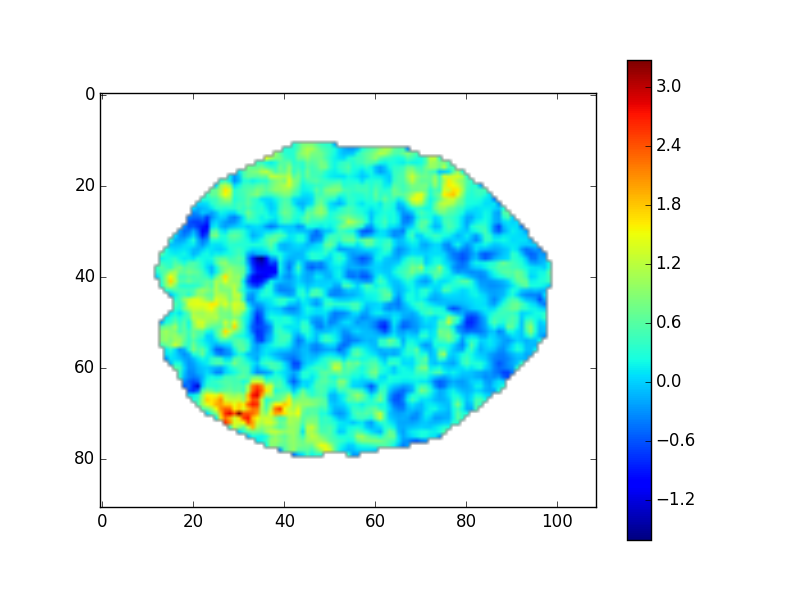
\includegraphics[width=0.7\textwidth]{4_CAT}}
    \caption{Figure4: CAT 4}
           
Next, we want to investigate the cat and every other regressor. 
According to the two graphs, we saw the lower region of the brain seems correspond very well to cat. Therefore, we make a new hypothesis again:  viewing a picture of an animal certain part of brain responds to animal. Since the two graphs have different scale, we have to compare the cat regressor and every other category regressor at the same scale.



\subsection{Cat vs Everything}

\begin{housevsface}
  \centering
    \reflectbox{%
      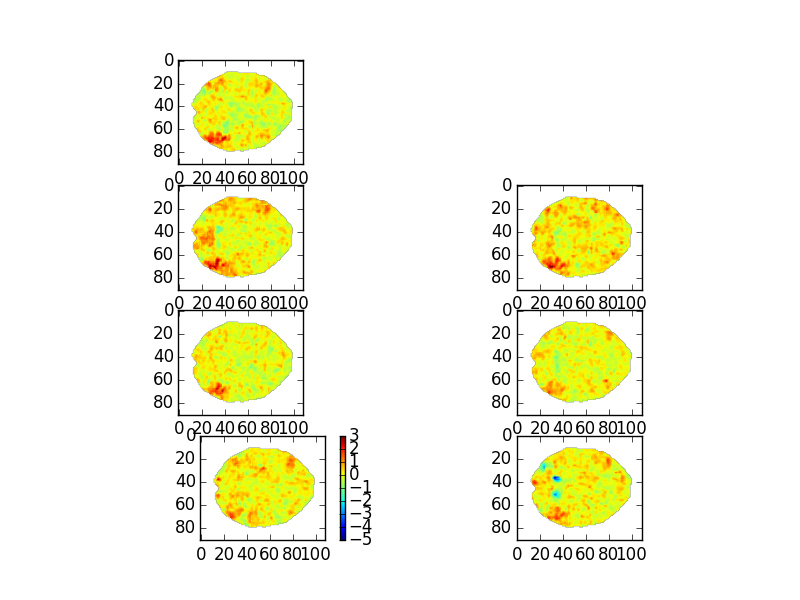
\includegraphics[width=1.2\textwidth]{cat_everything}}
    \caption{Figure5: Cat vs Everything}
           
           
According to the graph, it is clear to see that each graph has a red dot at lower region of the brain. Hence, we should accept our hypothesis, and we can make a conclusion that the regions strongly responds the animal picture.

\end{housevsface}


\subsection{Correlation}

\begin{housevsface}
After getting beat from run1, we want see the correlation between  region of the brain that react strongly to one category and not to other category. Here we want to show that the correlation is exactly same interpretation  of t_map. 
  \centering
    \reflectbox{%
      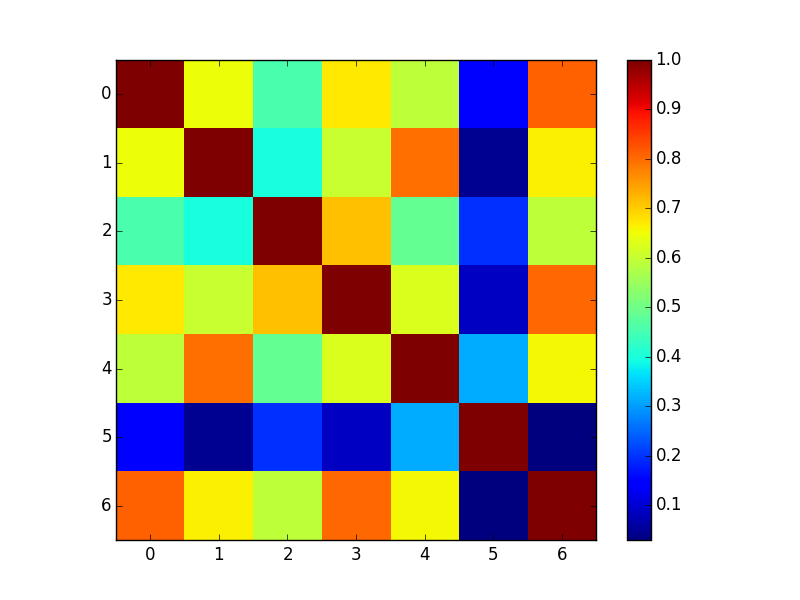
\includegraphics[width=1\textwidth]{1_correlation}}
        \caption{Figure7: Correlation 1}
\end{housevsface}



\subsection{More Corelation}

\begin{housevsface}
  \centering
    \reflectbox{%
      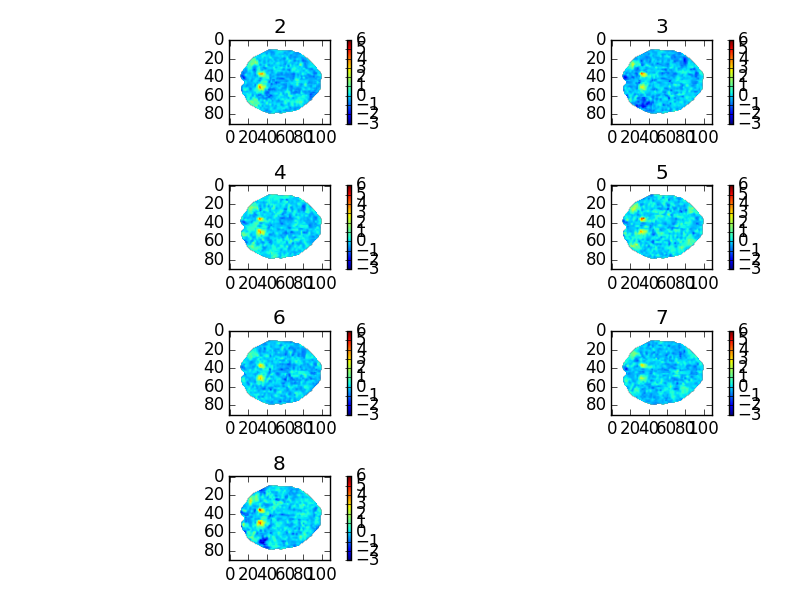
\includegraphics[width=1.2\textwidth]{house_everything}}
    \caption{Figure8: House vs Everything}
           
According to the house vs. everything graph, it is harder to see the red point from t-map between house and chair than other categories. Also, Beta chair minus Beta house has lower correlation than other two categories according to the number 1 correlation on figure 7. Therefore,  the correlation is exactly same interpretation  of t-map
\end{housevsface}

\subsection{}


\section{Results}

\subsection{Discussion}


\bibliography{project}

\end{document}